\subsection{Understanding Bell's Proof}
\begin{frame}{Over 80 Years Apart}
  % Minipages for the images
  \begin{minipage}{0.48\textwidth}
    \centering
    
\includegraphics[width=0.8\linewidth]{images/einstein.jpeg}
    \par\vspace{0.2cm}
    \textbf{Albert Einstein}
  \end{minipage}
  \hfill
  \begin{minipage}{0.48\textwidth}
    \centering
    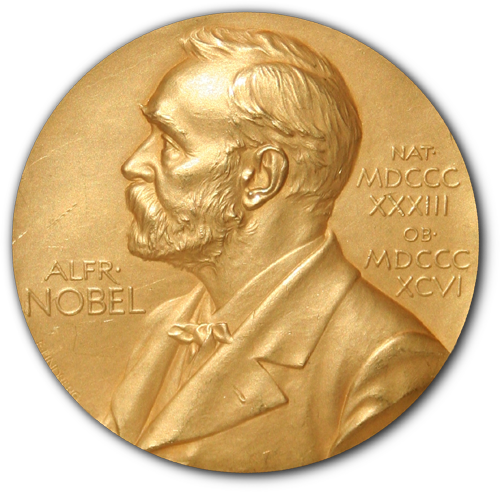
\includegraphics[width=0.8\linewidth]{images/nobel.png}
    \par\vspace{0.2cm}
    \textbf{Physics Nobel Prize}
  \end{minipage}
\end{frame}


\begin{frame}{Formulations vs Interpretations}

  \begin{minipage}[t]{0.43\textwidth} % Columna izquierda
    \begin{block}{Formulations of Quantum Mechanics}
      \vspace{0.2cm}
      \begin{itemize}
        \item Heisenberg's Matrix Mechanics
        \item Schrödinger's Wave Mechanics
        \item Hilbert Space Formalism (von Neumann)
        \item Bohmian Mechanics (Wave function decomposition: $R$ and $S$)
      \end{itemize}
    \end{block}
  \end{minipage}
  \hfill
  \pause
  \begin{minipage}[t]{0.53\textwidth} % Columna derecha
    \begin{block}{Interpretations of Quantum Mechanics}
    \vspace{0.2cm}
      \begin{itemize}
        \item Copenhagen Interpretation (Statistical, Collapse of the wavefunction)
        \item EPR Argument and Reality Criterion
        \item de Broglie-Bohm Interpretation (Hidden Variables, Deterministic)
        \item Quantum Potential and Nonlocality
        \item Bell's Theorem (Incompatibility with Local Realism)
      \end{itemize}
    \end{block}
  \end{minipage}

\end{frame}


\begin{frame}{Mathematische Grundlagen der Quantenmechanik}
  \begin{minipage}{0.44\textwidth}
    \centering
    \tikz\node[draw=purple!50, fill=purple!10, rounded corners=5pt, drop shadow] {
      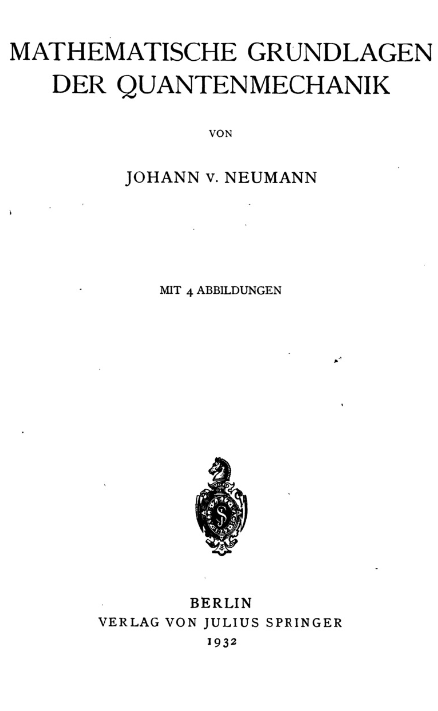
\includegraphics[width=0.6\linewidth]{images/neumann1.png}
    };
    \par\vspace{0.2cm}
    \small \textit{First German edition (1932)}
 
  \end{minipage}
  \hfill
  \begin{minipage}{0.44\textwidth}
    \centering
    \tikz\node[draw=purple!50, fill=purple!10, rounded corners=5pt, drop shadow] {
      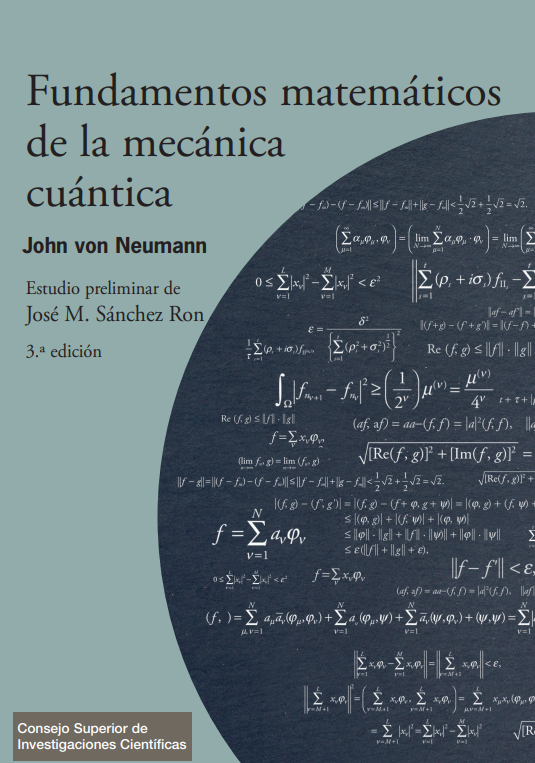
\includegraphics[width=0.65\linewidth]{images/neumann2.png}
    };
    \par\vspace{0.2cm}
    \small \textit{Spanish translation (CSIC, 3rd edition)}

  \end{minipage}
\end{frame}

% Slide 1: Axioms
\begin{frame}{Von Neumann's Axioms (Section IV.1)}
  Von Neumann does not start from the quantum formalism itself, 
  but rather establishes general axioms for the mean value of any 
  physical magnitude $R$ in a statistical ensemble, denoted as $V_m(R)$.  

  \pause
  \begin{itemize}
    \item[A'.] \textbf{Positivity:}  
    If a magnitude $R$ is intrinsically non-negative (e.g. the square of another quantity), then  
    \[
    V_m(R) \geq 0
    \]

    \pause
    \item[B'.] \textbf{Linearity:}  
    For arbitrary magnitudes $R, S, \dots$ and real numbers $a, b, \dots$:  
    \[
    V_m(aR + bS + \dots) = aV_m(R) + bV_m(S) + \dots
    \]
  \end{itemize}
\end{frame}

% Slide 2: Statistical Operator
\begin{frame}{Statistical Operator and Impossibility Result (Section IV.2)}
 
  Von Neumann proves a fundamental theorem:  

  \pause
  Any expectation value function $V_m(R)$ that satisfies axioms A' and B' 
  can be uniquely represented by a Hermitian, positive operator $U$, 
  called the \textit{statistical operator} (today: density matrix), via the trace formula:

  \pause
  \[
    V_m(R) = \mathrm{Tr}(UR)
  \]
\end{frame}

\begin{frame}{Conditions for a Hidden-Variable System}
  In the hidden-variable hypothesis, any physical magnitude $R$ 
  must satisfy the following conditions:

  \pause
  \begin{enumerate}
    \item \textbf{Eigenvalue Condition:}  
    The expectation value of any magnitude $R$ must coincide with one of its possible values (eigenvalues).  
    \[
      V_m(R) \in \{\text{eigenvalues of } R\}
    \]

    \pause
    \item \textbf{Dispersion-Free Condition:}  
    The variance of any magnitude $R$ must vanish, i.e.  
    \[
      V_m(R^2) = [V_m(R)]^2
    \]
  \end{enumerate}
\end{frame}

\begin{frame}{Von Neumann's Impossibility Proof}
  The core of von Neumann's argument is to show that there is no statistical operator $U$ 
  (and therefore no expectation-value function $V_m(R)$) that can simultaneously satisfy 
  the linearity hypothesis (B') and the condition of absence of dispersion for all observables.

  \vspace{0.5cm}

  \[
    V_m(RS) + V_m(SR) = 2\,V_m(R)\,V_m(S)
  \]

  \vspace{0.5cm}

  For non-commuting observables ($[R,S]\neq 0$), there is in general no assignment 
  of values $V_m(\cdot)$ that can satisfy this for all operators.
\end{frame}



\begin{frame}{Bhom And Hidden Variables}
  % Minipages for the images
  \begin{minipage}{0.48\textwidth}
    \centering
    
\includegraphics[width=0.8\linewidth]{images/einstein.jpeg}
    \par\vspace{0.2cm}
    \textbf{Albert Einstein}
  \end{minipage}
  \hfill
  \begin{minipage}{0.48\textwidth}
    \centering
    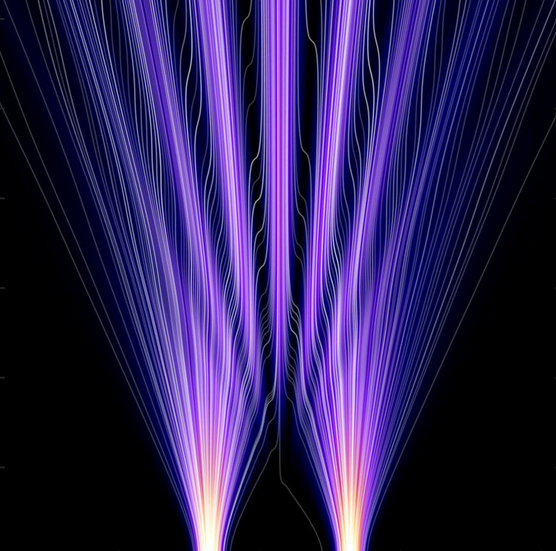
\includegraphics[width=0.9\linewidth]{images/Bhom.png}
    \par\vspace{0.2cm}
    \textbf{Bhom Trayectories}
  \end{minipage}
\end{frame}


\begin{frame}{Bhom Hidden Variables Papers}
  \begin{minipage}{0.49\textwidth}
    \centering
    \tikz\node[draw=purple!50, fill=purple!10, rounded corners=5pt, drop shadow] {
      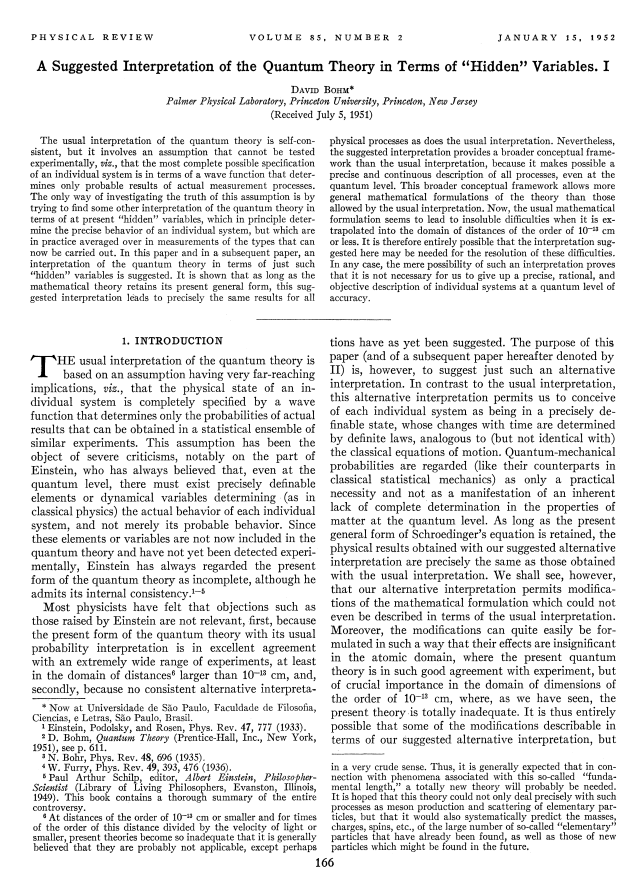
\includegraphics[width=0.7\linewidth]{images/bhompaperI.png}
    };
    \par\vspace{0.2cm}
    \small \textit{Hidden Variable I (1951)}
 
  \end{minipage}
  \hfill
  \begin{minipage}{0.49\textwidth}
    \centering
    \tikz\node[draw=purple!50, fill=purple!10, rounded corners=5pt, drop shadow] {
      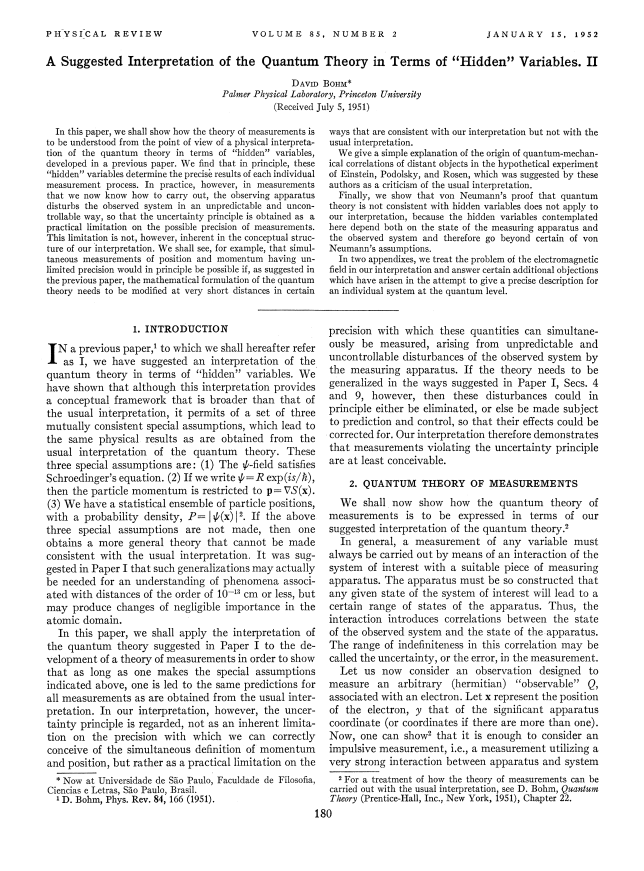
\includegraphics[width=0.7\linewidth]{images/bhompaperII.png}
    };
    \par\vspace{0.2cm}
    \small \textit{Hidden Variables II (1951)}

  \end{minipage}
\end{frame}

%---------------------------------------------------------
\begin{frame}{Bohmian Mechanics: Wave Function in Polar Form}

  \textbf{Starting Point: Time-Dependent Schrödinger Equation}
  \[
    i\hbar \frac{\partial \psi}{\partial t} 
      = -\frac{\hbar^2}{2m}\nabla^2\psi + V(\mathbf{x},t)\psi
  \]

  \pause

  \textbf{Polar Decomposition of the Wave Function}
  \[
    \psi(\mathbf{x},t) = R(\mathbf{x},t)\,e^{\tfrac{i}{\hbar}S(\mathbf{x},t)}, 
    \quad R \geq 0,\; S\in \mathbb{R}
  \]

  \pause

  This representation will split Schrödinger’s equation into two coupled \emph{real} equations:  
  a continuity equation and a Hamilton–Jacobi–like equation.  

\end{frame}

%---------------------------------------------------------
\begin{frame}{Bohmian Mechanics: Continuity and Quantum Potential}

  \textbf{Continuity Equation (Probability Conservation)}
  \[
    \frac{\partial P}{\partial t} 
      + \nabla\!\cdot\!\big(P\,\tfrac{\nabla S}{m}\big) = 0, 
    \qquad P = R^2
  \]

  \pause

  \textbf{Modified Hamilton–Jacobi Equation}
  \[
    \frac{\partial S}{\partial t} 
      + \frac{(\nabla S)^2}{2m} 
      + V(\mathbf{x},t) 
      + U(\mathbf{x},t) = 0
  \]
\end{frame}
  

\begin{frame}{Bohmian Mechanics: Continuity, Quantum Potential and Motion}

  \textbf{Quantum Potential}
  \[
    U(\mathbf{x},t) = -\frac{\hbar^2}{2m}\,\frac{\nabla^2 R}{R}
  \]

  \pause

  \textbf{Guidance Equation (Deterministic Trajectories)}
  \[
    \mathbf{p} = \nabla S(\mathbf{x},t), 
    \qquad \mathbf{v} = \frac{\nabla S}{m}
  \]

  \pause

  \textbf{Equation of Motion (Newtonian Form with Quantum Force)}
  \[
    m \frac{d^2 \mathbf{x}}{dt^2} = - \nabla \Big( V(\mathbf{x}) + U(\mathbf{x},t) \Big)
  \]

\end{frame}



%---------------------------------------------------------
\begin{frame}{Statistical Predictions in Bohmian Mechanics}

  \textbf{Determinism vs. Statistics}


  Although Bohm’s theory is deterministic for single systems,  
  it reproduces all statistical predictions of standard quantum mechanics  
  under three key assumptions:

  \pause
  \begin{enumerate}
    \item The field $\psi$ satisfies the Schrödinger equation.  
    \pause
    \item The particle’s momentum is always given by $p = \nabla S(\mathbf{x})$.  
    \pause
    \item In practice, we cannot predict or control the exact initial position,  
          so we work with an ensemble with probability density:
          \[
            P(\mathbf{x}) = R^2 = |\psi(\mathbf{x})|^2
          \]
  \end{enumerate}

\end{frame}

%---------------------------------------------------------
\begin{frame}{Consistency of the Statistical Postulate}

  \textbf{Continuity Equation Ensures Born’s Rule Preservation}

  \pause
  Starting from the polar decomposition, the continuity equation is:
  \[
    \frac{\partial P}{\partial t} + \nabla \cdot (P \mathbf{v}) = 0,
    \qquad \mathbf{v} = \frac{\nabla S}{m}
  \]

  \pause
  This guarantees that if $P(\mathbf{x},t_0) = |\psi(\mathbf{x},t_0)|^2$  
  at one instant, then $P(\mathbf{x},t) = |\psi(\mathbf{x},t)|^2$  
  for all later times.

  \pause
  \textbf{Interpretation:}  
  Probability is not fundamental but reflects ignorance of initial conditions,  
  just as in classical statistical mechanics.  

\end{frame}


%---------------------------------------------------------
\begin{frame}{Quantum Potential in Many-Body Systems}

\textbf{Extension to $n$ particles}

\pause
For a system of $n$ particles, the wavefunction is:
\[
\psi(x_1, x_2, \dots, x_n, t) = R(x_1, \dots, x_n,t)\, e^{\tfrac{i}{\hbar} S(x_1, \dots, x_n,t)}
\]

\pause
The quantum potential generalizes to:
\[
U(x_1, \dots, x_n) \;=\; -\frac{\hbar^2}{2m} \, \frac{\sum_i \nabla_i^2 R}{R}
\]

\pause
\textbf{Key feature:} $U$ depends on the coordinates of \emph{all} particles simultaneously.  

\end{frame}

%---------------------------------------------------------
\begin{frame}{Nonlocality and Entanglement in Bohm's Theory}

\textbf{Implications of the many-body quantum potential:}


\begin{itemize}
  \item The force on particle $i$,
  \[
  \mathbf{F}_i = -\nabla_i U,
  \]
  depends instantaneously on the positions of all other particles.
  \pause
  \item This represents an effective "many-body force" that is inherently \textbf{nonlocal}.
  
  \item In entangled states, the correlations predicted by quantum mechanics emerge naturally from this nonlocal potential.
  
  \item Thus, Bohm’s theory is \textbf{causal but nonlocal}, consistent with the EPR scenario.
\end{itemize}

\end{frame}

\begin{frame}{Bell 1964 Paper}
  \begin{center}
    \tikz\node[draw=blue!50, fill=blue!10, rounded corners=5pt, drop shadow] {
      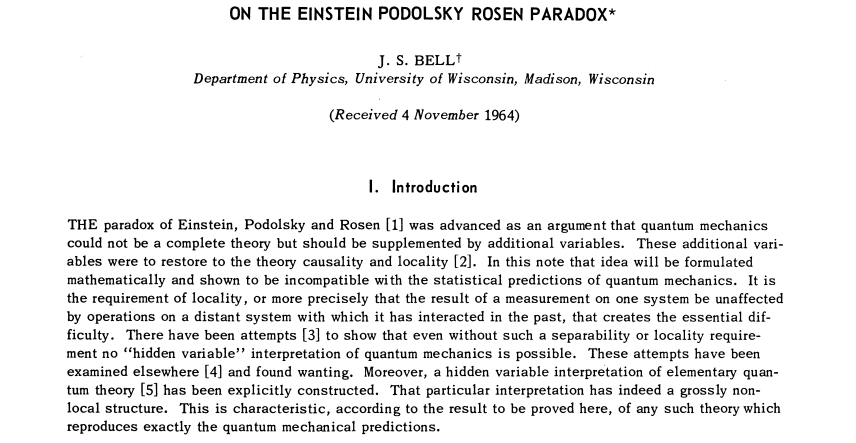
\includegraphics[width=0.8\linewidth]{images/bell1964.png}
    };
    \par\vspace{0.3cm}
    \small \textit{On the Einstein Podolsky Rosen Paradox (1964)}
  \end{center}
\end{frame}

%---------------------------------------------------------
% SLIDE 1: Fundamental Assumptions by Bell
\begin{frame}{Fundamental Assumptions of Bell}

\begin{itemize}
  \item \textbf{Hidden variables:} Each particle pair has a set of parameters $\lambda$ that determines measurement outcomes locally. \pause
  \item \textbf{Measurement results:} $A(a,\lambda), B(b,\lambda) \in \{+1,-1\}$ represent outcomes along directions $a$ and $b$. \pause
  \item \textbf{Perfect anticorrelation:} If $a=b$, then $A(a,\lambda) = -B(a,\lambda)$, consistent with quantum prediction $P(a,a)=-1$. \pause
  \item \textbf{Local correlation:} 
  \[
    P(a,b) = \int d\lambda\, \rho(\lambda)\, A(a,\lambda) B(b,\lambda)
  \]
  where $\rho(\lambda)$ is the probability distribution over the hidden variables. \pause
  \item \textit{Interpretation: correlations are determined solely by local properties of the particles and their hidden variables.}
\end{itemize}

\end{frame}

%---------------------------------------------------------
% SLIDE 2: Intermediate Steps of the Derivation
\begin{frame}{Bell Derivation: Key Intermediate Steps}

\begin{enumerate}
  \item \textbf{Rewrite using anticorrelation:}  
  \[
    P(a,b) = - \int d\lambda\, \rho(\lambda) A(a,\lambda) A(b,\lambda)
  \]

  \item \textbf{Comparing three directions:}  
  \[
    P(a,b)-P(a,c) = - \int d\lambda\, \rho(\lambda) \big[ A(a)A(b) - A(a)A(c) \big]
  \] \pause

  \item \textbf{Regroup using $A(b)^2=1$:}  
  \[
    P(a,b)-P(a,c) = - \int d\lambda\, \rho(\lambda) A(a)A(b) \big[ 1 - A(b)A(c) \big]
  \] 
  \textit{The difference in correlations depends on how particle 2’s “instructions” change between $b$ and $c$.}
\end{enumerate}

\end{frame}

%---------------------------------------------------------
% SLIDE 3: Final Inequality and Physical Meaning
\begin{frame}{Bell Inequality and Physical Meaning}

\[
|P(a,b) - P(a,c)| \le 1 + P(b,c)
\] \pause

\begin{itemize}
  \item $P(a,b)$: correlation measured between results along $a$ and $b$. \pause
  \item $P(a,c)$: correlation measured between $a$ and $c$. \pause
  \item $P(b,c)$: correlation between directions $b$ and $c$. \pause
  \item \textbf{Physical interpretation:} No local realistic theory can produce correlations stronger than this bound. \pause
  \item Violation of this inequality by quantum predictions implies:
    \begin{itemize}
      \item Realism and locality cannot both hold simultaneously. 
      \item Measurement outcomes are correlated in a nonlocal manner via entanglement.
    \end{itemize}
\end{itemize}

\end{frame}

\begin{frame}{Violation of Bell Inequality: Quantum Prediction}

\textbf{Quantum mechanics prediction for entangled particles:}

\vspace{-0.3cm}

\[
P_\text{QM}(\mathbf{a}, \mathbf{b}) = - \mathbf{a} \cdot \mathbf{b}
\]
\vspace{-0.3cm}

\pause

\textbf{Bell inequality :}

\vspace{-0.3cm}

\[
|P(\mathbf{a},\mathbf{b}) - P(\mathbf{a},\mathbf{c})| \le 1 + P(\mathbf{b},\mathbf{c})
\]

\vspace{-0.3cm}

\pause

\textbf{Specific setup:}  
\begin{itemize}
  \item Take a vector $\mathbf{c}$ “halfway” between $\mathbf{a}$ and $\mathbf{b}$.  
  \item Define angles: 
  \(\theta = \angle(\mathbf{a},\mathbf{c}) = \angle(\mathbf{c},-\mathbf{b})\)
\end{itemize}

\pause

\textbf{Substituting the quantum prediction:}

\vspace{-0.3cm}

\[
|- \mathbf{a} \cdot \mathbf{b} - (- \mathbf{a} \cdot \mathbf{c})| 
\le 1 - \mathbf{c} \cdot \mathbf{b} 
\quad \Rightarrow \quad 
|\cos(2\theta) - \cos(\theta)| \le 1 - \cos(\theta)
\]

\end{frame}



\begin{frame}{Explicit Violation for Small Angles}

\textbf{Approximations for small angles $\theta \ll 1$:}
\[
\cos(\theta) \approx 1 - \frac{\theta^2}{2}, \quad 
\cos(2\theta) \approx 1 - 2\theta^2
\]

\pause

\textbf{Bell inequality becomes:}
\[
| \cos(2\theta) - \cos(\theta) | \le 1 - \cos(\theta)
\quad \Rightarrow \quad
|(1 - 2\theta^2) - (1 - \frac{\theta^2}{2})| \le \frac{\theta^2}{2}
\]

\pause

\textbf{Simplifying:}
\[
\frac{3}{2}\theta^2 \le \frac{1}{2} \theta^2
\]

\pause

\textbf{Conclusion:}  
This inequality is \textbf{false} for any $\theta \neq 0$, demonstrating that 
\textbf{quantum mechanics predictions violate Bell’s inequality}.  

\end{frame}


\begin{frame}{Bell’s Refutation of von Neumann (1966)}

\begin{minipage}{0.65\textwidth}
\textbf{Bell’s Conceptual Criticism:}
\begin{itemize}
  \item Von Neumann’s \textbf{linearity assumption}: 
   \vspace{-0.4cm}

  \[
    V_m(aR+bS) = aV_m(R) + bV_m(S)
  \]

  \vspace{-0.3cm}
  \pause
  \item Imposed even on dispersion-free states.  
  \pause
  \item Bell argued this is \textbf{unjustified for non-commuting observables}.  
  \pause
  \item Example: measuring $\sigma_x + \sigma_y$ is not the same as separately measuring $\sigma_x$ and $\sigma_y$.  
  \pause
  \item Therefore, von Neumann’s proof excludes only a very restrictive class of hidden-variable theories.  
  \pause
  \item Bohm’s 1952 theory escapes because it is \textbf{contextual}.  
\end{itemize}
\end{minipage}
\hfill
\begin{minipage}{0.33\textwidth}
  \centering

  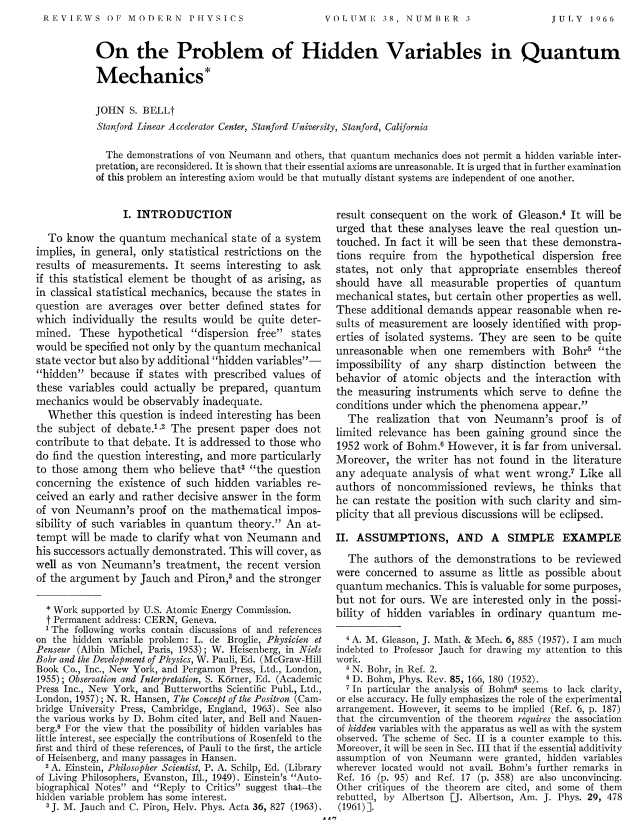
\includegraphics[width=\textwidth]{images/bell1966.png} \\
  \vspace{0.2cm}
  {\footnotesize Bell, J.S. \\
  \emph{On the problem of hidden variables in QM} (1966)}
\end{minipage}

\end{frame}




\begin{frame}{The CHSH Inequality}

\begin{minipage}{0.58\textwidth}

\textbf{Defining the correlation function:}

\vspace{-0.5cm}

\[
E(a,b) = \langle A(a) \, B(b) \rangle, 
\quad A, B = \pm 1
\]

\pause

\vspace{-0.2cm}

\textbf{The CHSH combination:}

\vspace{-0.6cm}

\[
S = E(a, b) - E(a, b') + E(a', b) + E(a', b')
\]

\pause

\vspace{-0.3cm}

\textbf{Local realism constraint:}

\vspace{-0.5cm}

\[
-2 \leq S \leq 2
\]

\pause

\vspace{-0.3cm}

\textbf{Quantum mechanics prediction:}

\vspace{-0.6cm}

\[
|S| \leq 2\sqrt{2} \quad \Rightarrow \quad \text{Violation of local realism}
\]

\pause

\vspace{-0.3cm}


\textbf{Impact:}
\begin{itemize}
  \item The CHSH form was \textbf{experimentally testable}.  
  \item Enabled landmark tests (e.g. Aspect, 1982).  
\end{itemize}

\end{minipage}
\hfill
\begin{minipage}{0.36\textwidth}

\textbf{Why correlations matter:}

\begin{itemize}
  \item The values $E(a,b)$ come from \textbf{statistical counts} of coincident detections.  
  \item Individual outcomes are random, but correlations reveal hidden structure.  
  \item The strength of violation depends entirely on these \textbf{count-based correlations}.  
\end{itemize}

\end{minipage}

\end{frame}



\begin{frame}{Conclusions on Quantum Entanglement}

\begin{itemize}
  \item EPR raised the dilemma about the \textbf{completeness} of quantum mechanics.  
  \pause
  \item Bell turned the \textbf{philosophical} debate into \textbf{mathematical and experimental predictions}.  
  \pause

  \item Entanglement reveals \textbf{nonlocal correlations}.  
  \pause
  \item Incompatible with classical \textbf{realism} and \textbf{locality}.  
\end{itemize}

\end{frame}


